\documentclass[12pt,preprint]{aastex}

%\documentclass[iop,apjl]{emulateapj}
\usepackage{amsmath}
%\bibliographystyle{hapj}


\usepackage{graphicx}
\usepackage{natbib}
%\usepackage{colortbl}
\newcommand{\vdag}{(v)^\dagger}
\newcommand{\myemail}{m.morscher@u.northwestern.edu}
%\usepackage{subfigure}
\usepackage{epsfig}
%\usepackage{subfig}
%\usepackage{multirow}
%\usepackage{array}

\usepackage{caption}
\usepackage{subcaption}
%\renewcommand{\topfraction}{0.85}
%\renewcommand{\textfraction}{0.1}


%\shorttitle{Black Holes in Star Clusters}
%\shortauthors{Morscher et al.}




\begin{document}

\title{Stellar-Mass Black Holes in Globular Clusters}
  
\author{Meagan Morscher, Carl Rodriquez, Stefan Umbreit, and Frederic A.\ Rasio}

\affil{Center for Interdisciplinary Exploration and Research in
  Astrophysics (CIERA), and Department of Physics and Astronomy,
  Northwestern University, 2145 Sheridan Road, Evanston, IL 60208,
  USA.}

\email{m.morscher@u.northwestern.edu}
\email{s-umbreit@northwestern.edu}
\email{rasio@northwestern.edu}



\begin{abstract}
We investigate the dynamical evolution of globular clusters containing a large number of stellar-mass BHs. Our main goal is to see whether it is possible for clusters to retain a significant number of BHs for $\sim 10\,$ Gyr and still resemble the Milky Way's population of old globular clusters (GCs). We use a Monte Carlo method, which allows us to model large-$N$ clusters with all the relevant physics required to describe these systems accurately. We present a grid of 42 realistic Monte Carlo simulations that span a range of initial physical properties. We find that under standard assumptions for initial cluster models, including the initial BH population, all of our models that survive to $\sim 10\,$ Gyr still contain a significant number ($\gtrsim\, 50$) of BHs at the end of the simulation. This population of retained BHs produces a heating effect which prevents the cluster cores from collapsing down to the sub-parsec scale that is typical for MW GCs. However, we urge the use of caution when using measured core radii as a means for comparing models to real MW clusters.
Our results suggest the need to revisit our understanding of BH formation and observational studies of BHs, including the BH mass function as well as the strength of supernova kicks for BHs.
	% ABSTRACT STILL NEEDS SOME WORK

\end{abstract}

%%%%%%%%%%%%%%%%%%%%%%%%%%%%%%%%%%    INTRODUCTION    %%%%%%%%%%%%%%%%%%%%%%%%%%%%%%%


\section{Introduction}

Massive star clusters should form $\sim 100\, -\, 1000$ stellar-mass black holes (BHs) through normal stellar evolution, and as long as BH birth kicks are sufficiently low, most should be retained in the cluster initially. 
[SHOULD I REMOVE ITALICIZED SECTION? \emph{Through dynamics, these BHs can become members of binary systems with either stellar or dark remnant companions, and evolve to produce X-ray binaries (XRBs) or merging compact object binaries, which will be detectable by future gravitational wave (GW) observatories (e.g. LIGO; \citealt{HarryLIGO2010}). These systems can, in theory, be found either inside of clusters or in the field. It is well known that the formation rate per unit mass of XRBs is orders of magnitude larger in clusters than it is in the field (e.g., \citealt{Pooley2003}), which suggests that stellar dynamics must play an essential role in producing XRBs in present day clusters.} ]
Since the early nineties, however, theoretical arguments, simulations and observations have all suggested that old GCs should have very few ($\lesssim1$) BHs at present. Early studies (\citealt{Kulkarni1993}, \citealt{Sigurdsson1993}) predicted from analytic arguments that the BHs, being heavier than other stars, should rapidly segregate to the cluster center through dynamical friction against the lighter background stars and eventually succumb to the so-called Spitzer instability \citep{Spitzer1969, Kulkarni1993}. If this happens, the BHs will form a dense subsystem within the cluster core that consists primarily of BHs, and is dynamically decoupled from the cluster. The small-$N$ sub-cluster of BHs has a very short relaxation time, so it will undergo its own core collapse, begin to form hard binaries through three-body interactions, and subsequently begin ejecting single and binary BHs. The system of BHs will evaporate within a timescale of a few Gyr, leaving behind a cluster essentially devoid of BHs. Other theoretical studies confirmed this idea through idealized simulations (e.g., \citealt{PortegiesZwart2000}, \citealt{OLeary2006}). Over the last several years, however, our understanding about BHs in dense star clusters has shifted quite dramatically.

This old story began to change when the first BH X-ray binary was detected inside of an old GC in an external galaxy, NGC 4472 \citep{MaccaroneNature2007}. Several more BH XRBs were subsequently discovered inside of GCs (\citealt{Barnard2011}, \citealt{Shih2010}). Recently, \cite{Strader2012} discovered \emph{two} BHs inside of the Milky Way GC M22. These BHs are the first ever to be found in a GC in our \emph{own} galaxy, as well as the first to be \emph{discovered} through radio observations. By assuming that these systems are BH-WD binaries, they used published theoretical calculations from \cite{Ivanova2010} to estimate the fraction of present-day BHs in GCs that are actively accreting from a WD companion. They estimate that the detection of two accreting BHs in M22 implies a true population of $\sim 5-100$ BHs.  The same group recently found another BH in a different galactic GC, M62, also through radio observations \citep{Chomiuk2013}. 

On the theoretical side, a few recent studies have provided hints that old clusters might be able to retain BHs for many Gyr. \cite{Mackey2008} used $N$-body simulations of clusters with BHs to explain the radius-age trend in the Magellanic Cloud clusters. With models of varying initial BH retention, they found that a population of retained BHs could provide a heat source for some clusters, providing a possible explanation for the observed spread in the radii of observed Magellanic Cloud clusters. In some of these models, significant numbers of BHs (as many as $\approx 100$) were retained for $\sim$ 10 Gyr. 
%\cite{Moody2009} use semi-analytic calculations of the dynamics of BH-binary interactions in clusters to study the rate of BH mergers. They find that in their most massive and metal-rich clusters, 5\% of their BH-binaries are actually retained.
\cite{Sippel2013} present a scaled-down (in mass) direct $N$-body model of M22, known to host \emph{two} stellar-mass BHs. At an age of 12 Gyr, their model retains 16 BHs (about 1/3 of the initially-retained population), which is consistent with the prediction of \cite{Strader2012}. A Monte Carlo study by \cite{Morscher2013} found that some clusters may retain as many as \emph{hundreds} of BH for 12 Gyrs.  The long-term survival of such a large number of BHs is explained by the fact that the BHs do not become Spitzer unstable on the whole, but rather the majority of BHs remain well mixed with the rest of the cluster throughout the entire 12 Gyr evolution.

A very different study by \cite{Breen2013} focused on the evolution of two-component clusters, with a population of BHs co-existing within a cluster of light stars. They provide theoretical calculations as well as direct $N$-body simulations which both suggest that the flow of energy in the system is ultimately determined by the cluster. In this way, the rate of energy production in the BH subsystem as well as its evaporation rate is regulated by the cluster. This implies that BHs can survive for much longer than previously thought (i.e., for $\sim 10\, T_{rh,i}$, where $T_{rh,i}$ is the initial half-mass relaxation timescale) because their dynamical evolution happens on the relaxation timescale of the \emph{cluster}, rather than that of the BH subsystem. This result suggests that the long-standing belief that BHs will dynamically decouple from clusters may be incorrect, which would imply that the foundation for the argument that old clusters should be deplete of BHs is essentially shattered. [I SHOULD CHANGE THAT WORD - TOO STRONG]

The topic of BHs in clusters is still worthy of further discussion. While the theoretical arguments presented in \cite{Breen2013} are interesting, these two-component models cannot be directly compared to real GCs, which have a  broad spectrum of stellar and BH masses, as well as larger total cluster masses. Several more-realistic studies have now predicted the survival of at least some BHs (e.g., \citealt{Mackey2008, Morscher2013, Sippel2013}), but there is still no definitive answer as to \emph{how many} might actually be hiding in old GCs at present. 
In this paper, we present a large grid Monte Carlo simulations of realistic, large-$N$, Milky-Way-like cluster and address the question of retention of BHs and structural evolution of clusters with BHs.
%There is still no large grid of realistic, large-$N$, Milky-Way-like cluster models that have addressed the question of retention of BHs and structural evolution of clusters with BHs. In the present paper, we address this need with a set of realistic Monte Carlo GC simulations. 
The rest of the paper is organized as follows:  FILL IN!


\section{Monte Carlo Method}
\subsection{Overview of Method}
We use a Monte Carlo (MC) method for modeling the dynamical evolution of GCs.
While the direct $N$-body method is more exact than MC schemes, 
it can only simulate clusters with up to $N \sim 10 \times 10^5$ due to the
poor scaling with $N$ (computation time $\sim N^3$). In order to model large MW GCs
with initial $N$ up to $\sim 10^6$, we must employ a Monte Carlo (MC) technique. 
\emph{SHOULD I CUT ITALICIZED SECTION? In contrast to the direct $N$-body method, which directly integrates the equations 
of motion of all particles, the MC method, cluster evolution is approximated using the 
theory of two-body relaxation. Stellar orbits are not resolved on a dynamical
timescale. Instead, the constants of motion for each star, energy $E$ and angular 
momentum $J$, are tracked. On the relaxation timescale, many long-range,
weak gravitational scattering interactions among stars perturbs the stellar orbits, 
 leading to a flow of energy from the cluster core outwards, and driving 
 cluster evolution. In the MC method, this is treated with a single interaction
  among each pair of stars per time step, where this single effective interaction 
  represents the cumulative effect of many gravitational interactions over
   the time step.} In MC methods, computation time scales as 
   $\sim N$ log$N$, which makes it feasible to model large
 GCs and to study the evolution of rare objects, such as BHs.

Our MC implementation is a variation of the ``orbit-averaged Monte Carlo 
method" developed by \cite{Henon1971a} for solving the Fokker-Planck 
equation. The details of our method are described in \citealt{Joshi2000}, 
\citealt{Joshi2001}, \citealt{Fregeau2003}, \citealt{Fregeau2007} and 
\citealt{Chatterjee2010}. Here we highlight the most important details for
the present study. We treat the cluster on a star-by-star basis,
and therefore it is relatively straightforward to add physics, one layer at
a time. Stars and binaries are evolved according to the stellar
evolution fitting formulae and interacting binary evolution calculations
of SSE and BSE (\citealt{Hurley2000}, \citealt{Hurley2002}), with 
modifications to the stellar remnant formation prescription according
to \cite{Belczynski2002}, which produces BH masses in the range 
$\sim 5-30\, M_\odot$ for $Z=0.001$. Both neutron stars (NS) and BHs receive natal kicks
assumed to be generated by the asymmetric ejection of mass during 
a supernova explosion. N kicks are drawn from a Maxwellian
distribution with $\sigma$=265 km s$^{-1}$. BHs are expected to receive
much lower velocity kicks (see \citealt{Wong2012} and references therein),
 and thus we follow the prescription of \cite{Belczynski2002} to reduce the
 kick magnitude according to the amount of material that falls back onto the 
 final BH after the supernova explosion. BHs that form via direct collapse 
 (i.e. all material falls back onto the BH) do not receive natal kicks.
BSE calculates the orbital evolution due to emission of GW radiation in compact
 object binaries, which is important for tracking the mergers of 
BH-BH binaries. Once a binary is ejected from the cluster, however, 
it is no longer evolved with our MC code.
For these systems, we estimate the merger time using a simplified timescale 
for GW in spiral in the weak field limit \citep{Peters1964} based on the system's
properties at the time of ejection.

In addition to two-body relaxation, we account for
strong binary interactions between either a binary and a single star [BS]
or two binaries [BB]. Strong interactions are calculated in a MC fashion
based on the cross-section for a close interaction between the pair of 
neighboring objects, and these interactions are then integrated 
directly using FEWBODY. These resonant binary interactions allow for many
important effects within binary systems, such as exchanges, binary hardening,
ionization, and ejections, all of which are relevant for the evolution of BHs in clusters.


\subsection{New Physics: Three-body Binary Formation}

We have recently implemented a simplified prescription for three-body 
binary formation, a process that is expected to produce an important 
population of hard BH-binaries 
\citep{Kulkarni1993, Sigurdsson1993, PortegiesZwart2000,OLeary2006,  
Banerjee2010}, and is therefore extremely important for this study. 
If three single stars experience a close resonant encounter, it is possible for two
of the stars to become gravitationally bound to one another, with the third star 
carrying away the extra energy. The probability
of binary formation is usually quite low, and realistically only becomes possible 
under the extreme conditions expected at the core of a cluster which has been driven
to collapse by a population of BHs. We only allow BHs to form binaries, since they 
are most likely to be found near the cluster center where the density is large 
enough for binary formation to occur. We restrict our attention to 
dynamically hard binaries, as only hard binaries are expected to survive \citep{Heggie1975}.
Our simplified prescription relies on the calculation of the rate at which 
three neighboring single BHs will form a hard binary. Using the calculated rate
and the current timestep, we can estimate the probability that the three-body
 system will result in binary formation, and then use MC sampling to select which systems
  will actually form a new binary.

% This is copied from my ApJ letter...must rephrase
Our prescription is similar to that of 
\citet{Ivanova2005}, \citet{Ivanova2010}, and \citet{OLeary2006},
where the rate is expressed as a function of binary hardness,
which ratio of the binding energy of the binary to the average local stellar kinetic energy,
\begin{equation}
\eta = \frac{G \, m_1 \, m_2}{r_p \, <m> \, \sigma^2}.
\label{eq:eta}
\end{equation}
Here $m_1$ and $m_2$ are the masses of the two stars assumed to
form a binary, $r_p$ is their separation at pericenter, and <m>  and $\sigma$ are
the local average mass and velocity dispersion.

Keeping both the geometric and gravitational focusing contributions to
the cross-section (in contrast to \citealt{Ivanova2010}, where the
geometric part of the cross section for the third star to interact
with stars 1 and 2 is dropped), we construct an expression for the
rate of binary formation for the selected neighboring three stars.
 For local number density, $n$, and
average relative velocity at infinity, $v_{\infty}$, the rate at which
two stars ($m_1$ and $m_2$) form a binary with hardness $\eta \, \geq
\, \eta_{\rm min}$ through an interaction with a third star ($m_3$) is
given by
\begin{multline}
\Gamma(\eta \geq \eta_{min}) = \sqrt{2} \pi^2 n^2
      {v_{\infty}^{-9}} \\ \times (m_1 + m_2)^5 \eta_{\rm min}^{-5.5} (1 + 2
      \eta_{\rm min}) \\ \times \left[ 1+2 \eta_{\rm min} \left( \frac{ m_1 + m_2 +
            m_3}{m_1 + m_2 } \right) \right].
\label{eq:Gamma}
\end{multline}
When our scheme predicts that a binary should form, we choose a
value for $\eta$ from a distribution according to the differential
rate, d$\Gamma$/d$\eta$, with lower limit $\eta_{\rm min}$. 
The rest of the properties of the system are calculated from 
conservation of momentum and energy. 



As we expect only dynamically hard binaries to survive
\citep{Heggie1975}, we only consider the formation of hard binaries
with $\eta \geq 5 = \eta_{\rm min}$.  We allow three-body binary
formation only for BHs.  When forming a three-body binary, we choose a
value for $\eta$ from a distribution according to the differential
rate, d$\Gamma$/d$\eta$, with lower limit $\eta_{\rm min}$. The rest
of the properties of the system are calculated from conservation of
momentum and energy.
% End section copied from ApJ letter

\subsection{Comparison to $N$-body Models}
BREEN  HEGGIE COMPARISON


\section{Initial Conditions}

We have calculated the dynamical evolution of 26 cluster models with different initial conditions, but all initialized as King models. The main parameters we have chosen to value are the initial number of stars $N$ ($N$=$2 \times 10^5$ and $N$=$8 \times 10^5$), the initial King concentration parameter ($W_o$=2, 5, 7) and the metallicity, which in our models correspond to three different galactocentric distances ($R_G$) ($Z$=0.005 at $R_g$=2 kpc, $Z$=0.001 at $R_g$=8 kpc and $Z$=0.0001 at $R_g$=20 kpc). We have chosen to correlate $Z$ and $R_g$ because there is a known correlation with GC metallicity and galactocentric distance, with the GCs at smaller $R_g$ having higher metallicity (ref?) . All of the permutations of these initial conditions gives us 18 models. All of these 18 models have the same initial virial radius $R_v$=2 pc, binary fraction $f_b$=10\% and initial mass function (IMF; Kroupa 2001 ranging from 0.1 -- 100$\, M_\odot$). In addition to the grid of 18 models, for our canonical model at each $N$, we ran one model with a larger initial virial radius ($R_v$=4 pc), with larger and smaller binary fraction (1\% and 50\%), and with a higher concentration ($W_o$=11). We do not attempt to reproduce the distribution of GCs with different properties, but rather our goal is to see whether GCs with many BHs can evolve into $\sim 10\, \rm Gyr$ old clusters that are consistent with the properties of MW GCs. We evolve all of our models to 12 Gyr, which is a typical age for MW GCs. Our initial models are give in Table ***.

All models with $N = 2 \times 10^5$ have initial total mass of $M_{\rm tot} = blah \times 10^5\, M_\odot$, and form $\sim xx$ BHs HOW MANY BHS- DO THEY HAVE ROUGHTLY SAME NUMBER FOR EACH N (OR DEPENDS ON METALLICITY). All models with $N = 8 \times 10^5$ have initial total mass of $M_{\rm tot} = blah \times 10^5\, M_\odot$, and form $\sim xx$ BHs. Note that some of the BHs that are formed through stellar evolution are ejected immediately upon formation by a natal kick. Details about the initial population of BHs, including the fraction of BHs retained initially, are given in table ****.

\subsection{Initial Black Hole Populations}

\section{Results}


\section{Evolution of BHs in Clusters}
We now describe the overall evolution common to all of our models. The BHs form very early (within a few Myr) and with masses larger than that of typical stars, the BHs begin to sink due to dynamical friction against the light background. This occurs on a timescale of BLAH, as can be seen in figure BLAH, shows the lagrange radii for the BHs compared to the rest of the cluster (excluding the BHs). The most massive BHs tend to sink the most quickly, driving central collapse in the cluster. Note that only a small subset of the BHs sink dramatically, with most of the BHs remaining well mixed with the rest of the cluster. (SHOW LAGRANGE RADII, CHECK WHAT I'M SAYING HERE). At this point, the core reaches high enough density that the rate of binary interactions starts to increase. Since the core is dominated by BHs, it is these BHs that are the primary source of interactions. These strong binary interactions lead to the ejection of BH ejections, which typically begin soon after the collapse of the BH subpopulation. $\sim TIME??$
FIG: LAGRANGE RADII FOR TWO MODELS - N=2E5 AND N=8E5
FIG: NUMBER OF BINARY INTERACTIONS.

\

\section{Comparison to Observation}
\subsection{Basic Properties}

We compare the properties of our models at 12 Gyr to the observed properties of MW GCs as taken from the Harris catalog. The core- and half-mass radius are converted from angular units to physical units (pc) using the distance as reported in Harris.  We have calculated the central luminosity density using the central **BLAH** stars. The luminosity of our stars is determined automatically by BSE. We convert the bolometric luminosity to V-band luminosity using **BLAH** and then calculate the luminosity density according to over the volume enclosed by the innermost **BLAH** stars. The half-light radius is defined as the radius that encloses half of the total cluster luminosity, and is determined using the calculated V-band luminosities.

\subsection{Core Radii}

One key observable property of GCs is the core radius, which is the...   We calculate the core radii for our models in a new way than is typically done for GCs. Typically, the core radius is determined by binning stars radially and constructing a surface brightness profile (SBP). The core radius is then either determined by fitting a king model to the SBP, or by finding the radius at which the luminosity density drops to half the central value. The problem with this is that, since the stars must be binned, there is always some degree of statistical noise. You want your bins to be small enough in radius that you can resolve your core, but small bin sizes increases the statistical noise. Often observers will remove the brightest stars, which can dominate the luminosity for the bin in which they reside. Since the brightest stars are rare, this introduces a large degree of bin-to-bin variation.

To avoid the noisiness that comes with binning, we chose to fit a King model to the \emph{cumulative} luminosity function, rather than the luminosity density.  Using King, an analytic approximation for a King model density profile, we integrated the formula for the surface luminosity over the surface area out to some distance $r$, which becomes the cumulative luminosity. For each model, we calculated the cumulative bolometric luminosity as a function of the radial coordinate $r$, and then fit the equation blah, which gave us the best fit values for the $\Sigma_o$ and $R_c$. We compared our results to that obtained from the SBP. The core radii determined with our new method agreed to within ~blah percent of the values based on the SBP. We show an example of the SBP and the cumulative luminosity function, as well as the determined $R_c$ values, for one of our models in figure BLAH.

\subsection{Results}

In figure BLAH we show the distribution of various cluster properties, including cluster mass $M_{\rm cl}$, the central luminosity density $\rho_{\rm c}$, core radius $r_{\rm c}$, and the ratio of core to half-light radius, $r_{\rm c} / r_{\rm h}$.  



In this figure, we have also marked the values of each of these quantities for all our models. We find that our models span the majority of the range of values for the MW GCs in terms of $M_{cl}$ and $\rho_c$. Our models do not quite reach the most massive and highest density end of the distribution, but this most likely has to do with the fact that our largest model has $N=8 \times 10^5$ stars. (brief justification for this here). When it comes to core radii, we find poor agreement with the MW population. Most MW GCs have a core radius less than 1 pc. In contrast, most of our models have core radii of several parsecs, with the smallest two $r_c$ values **list values here**. This discrepancy is explained by the large population of BHs that is retained over the entire evolution. While each cluster has ejected many BHs, they have held onto nearly as many. These BHs continue to interact with one another through strong binary scattering interactions, which lead to ejections of BHs. These ejections are a source of energy for the core, and thus the process causes significant core expansion.


\section{Discussion and Conclusions}




%%%%%%%%%%%%%%%%%%%%%%%%%%%%%%%%%%%%    FIGURES    %%%%%%%%%%%%%%%%%%%%%%%%%%%%%%%%
% central lum density histogram � GCs + models 
% cluster mass histogram � GCs + models 
% core radii histogram � GCs + models 
% rh/rc histogram � GCs + models 
% Rc vs Mcl � GCs + models
%




%\begin{figure}
%	\plotone{hist_rho_models_and_GCs.eps} 
%	\caption{Histogram of central luminosity densities ($L_{\odot}\, \rm pc^{-3}$) for observed GCs with values for our models indicated with red dashes. We see that our models span most of the range of observed central densities, missing only the very lowest and highest density tails of the distribution. (RUN NEW MODELS TO FILL THIS IN)
%	}
%
%	\label{fig:rho_hist}
%
%\end{figure}


%\begin{figure}
%	\plotone{./plots/rc_histogram_harris_models.eps}
%	\caption{Histogram of observed core radius, $r_c$ (left) and ratio of core to half light radius, $r_c\, /\, r_h$, for Milky Way GCs (Harris), along with the measured from our standard models, represented by tick marks on the x-axis. Red and blue ticks correspond to models with $N=2 \times 10^5$ and $N=8 \times 10^5$, respectively. Our models produce core radii that are significantly larger than most of the MW clusters. We do not produce any models with $r_c \leq 1$ pc. Also, our measured $r_c\, /\, r_h$ values are also on the large end for MW clusters.
%	}
%
%	\label{fig:rc_hist}
%
%\end{figure}


\begin{figure}
        \centering

        \begin{subfigure}[b]{0.5\textwidth}
                \includegraphics[width=\textwidth]{./plots/rc_histogram_harris_models.eps}
                \caption{}
                \label{fig:rc_hist}
        \end{subfigure}%
           \begin{subfigure}[b]{0.5\textwidth}
                \includegraphics[width=\textwidth]{./plots/rc_over_rh_histogram.eps}
                \caption{}
                \label{fig:rc_over_rh_hist}
        \end{subfigure}
       
       \caption{Histogram of observed core radius, $r_c$ (left) and ratio of core to half light radius, $r_c\, /\, r_h$, for Milky Way GCs (Harris), along with the measured from our standard models, represented by tick marks on the x-axis. Red and blue ticks correspond to models with $N=2 \times 10^5$ and $N=8 \times 10^5$, respectively. Our models produce core radii that are significantly larger than most of the MW clusters. We do not produce any models with $r_c \leq 1$ pc. Also, our measured $r_c\, /\, r_h$ values are also on the large end for MW clusters.}
 
 \end{figure}   



% BH MASS HISTOGRAMS FOR 2 MODELS
\begin{figure}
        \centering

        \begin{subfigure}[b]{0.5\textwidth}
                \includegraphics[width=\textwidth]{./plots/r5_bh_hist_all.eps}
                \caption{}
                \label{fig:r5_bh_hist}
        \end{subfigure}%
           \begin{subfigure}[b]{0.5\textwidth}
                \includegraphics[width=\textwidth]{./plots/r14_bh_hist_all.eps}
                \caption{}
                \label{fig:r14_bh_hist}
        \end{subfigure}
       
       \caption{BH mass functions for two different models:  n2e5\_w5\_r2\_Rg8\_z0.001 (left) and n8e5\_w5\_r2\_Rg8\_z0.001  (right)}
 
 \end{figure} 




% BH TIME EVOLUTION FIGURES
\begin{figure}
        \centering

        \begin{subfigure}[b]{0.5\textwidth}
                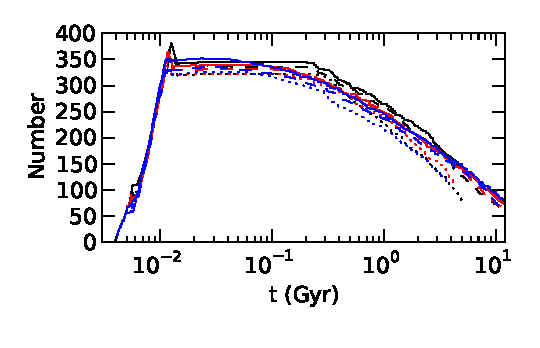
\includegraphics[width=\textwidth]{./plots/n2e5_bh_ret_timevolution.eps}
                \caption{r1}
                \label{fig:n2e5_bhs}
        \end{subfigure}%
           \begin{subfigure}[b]{0.5\textwidth}
                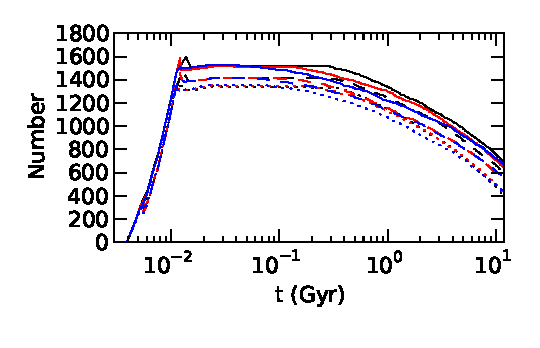
\includegraphics[width=\textwidth]{./plots/n8e5_bh_ret_timevolution.eps}
                \caption{r2}
                \label{fig:n8e5_bhs}
        \end{subfigure}
       
        \begin{subfigure}[b]{0.5\textwidth}
                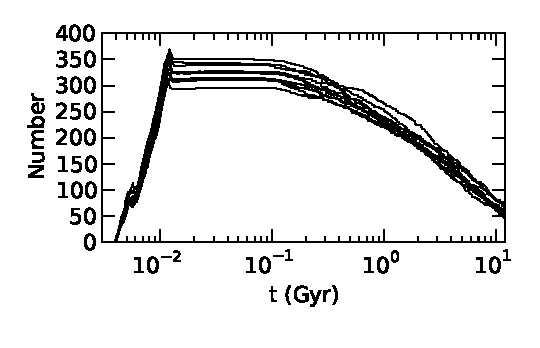
\includegraphics[width=\textwidth]{./plots/r5_repeat10_bh_ret_timevolution.eps}
                \caption{r2}
                \label{fig:repeat10_bhs}
        \end{subfigure}     
       
	% Add 'more_runs' and N=1.6e6 runs when done


       \caption{}
 \end{figure}    
   


% CLUSTER MASS TIME EVOLUTION FIGURES
\begin{figure}
        \centering

        \begin{subfigure}[b]{0.5\textwidth}
                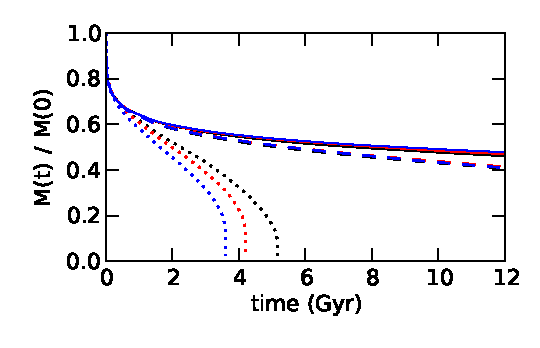
\includegraphics[width=\textwidth]{./plots/n2e5_mass_timeevolution.eps}
                \caption{r1}
                \label{fig:n2e5_mass}
        \end{subfigure}%
           \begin{subfigure}[b]{0.5\textwidth}
                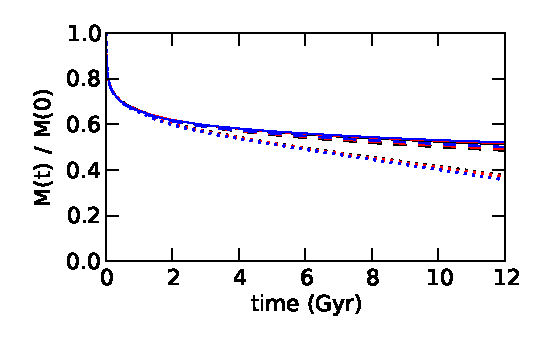
\includegraphics[width=\textwidth]{./plots/n8e5_mass_timeevolution.eps}
                \caption{r2}
                \label{fig:n8e5_mass}
        \end{subfigure}
       
        \begin{subfigure}[b]{0.5\textwidth}
                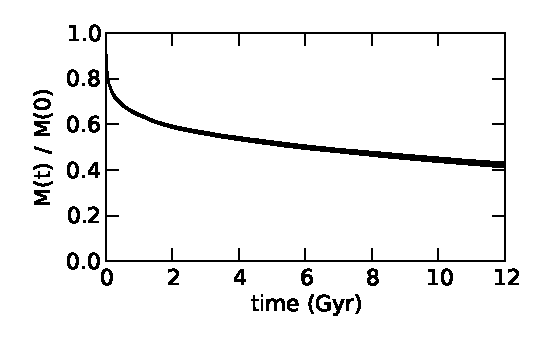
\includegraphics[width=\textwidth]{./plots/r5_repeat10_mass_timeevolution.eps}
                \caption{r2}
                \label{fig:repeat10_mass}
        \end{subfigure}     
       
	% Add 'more_runs' and N=1.6e6 runs when done


       \caption{}
 \end{figure}   




%\begin{figure}
%	\plotone{hist_rh_over_rc_models_and_GCs.eps}
%	\caption{
%	}
%
%	\label{fig:rh_over_rc_hist}
%
%\end{figure}
%
%
%
%\begin{figure}
%	\plotone{rc_vs_M_models_and_GCs.eps}
%	\caption{
%	}
%
%	\label{fig:rc_vs_M}
%
%\end{figure}



%%%%%%%%%%%%%%%%%%%%%%%%%%%%%%%%%%%%    TABLES    %%%%%%%%%%%%%%%%%%%%%%%%%%%%%%%%%
% 1. Initial properties � all models
% 2. Final properties � all models
% 3. Final BH stats � all models




\begin{deluxetable}{ccccccc}
%\rotate
%\tablecolumns{7}
\tabletypesize{\scriptsize}
%\tablewidth{0pc}
\tablecaption{Initial cluster properties. Columns are as follows: model name, initial $N$, initial cluster mass ($M_{\odot}$), initial theoretical (code defined) core radius (pc), initial half mass radius (pc), initial central mass density ($M_{\odot}/pc^3$), and initial binary fraction.}

\tablehead{
\colhead{model} & \colhead{$N$} & \colhead{$M$} & \colhead{$r_{c,code}$} & \colhead{$r_{h,code}$} & \colhead{$log(\rho_{c})$} & \colhead{$f_{b}$}   \\
\colhead{ } & \colhead{$(10^5)$} & \colhead{$(10^5 M_{\odot})$} & \colhead{(pc)} & \colhead{(pc)} & \colhead{$(M_{\odot}$/pc$^3)$} & \colhead{}
}

\startdata

n2e5\_w2\_r2\_Rg20\_z0.0005 & 2.0 & 1.36 & 0.951 & 1.698 & 4.47 & 0.1 \\
n2e5\_w2\_r2\_Rg8\_z0.001 & 2.0 & 1.36 & 0.951 & 1.698 & 4.47 & 0.1 \\
n2e5\_w2\_r2\_Rg2\_z0.005 & 2.0 & 1.36 & 0.951 & 1.698 & 4.47 & 0.1 \\
n2e5\_w5\_r2\_Rg20\_z0.0005 & 2.0 & 1.36 & 0.717 & 1.628 & 4.75 & 0.1 \\
n2e5\_w5\_r2\_Rg8\_z0.001 & 2.0 & 1.36 & 0.717 & 1.628 & 4.75 & 0.1 \\
n2e5\_w5\_r2\_Rg2\_z0.005 & 2.0 & 1.36 & 0.717 & 1.628 & 4.75 & 0.1 \\
n2e5\_w7\_r2\_Rg20\_z0.0005 & 2.0 & 1.36 & 0.449 & 1.624 & 5.25 & 0.1 \\
n2e5\_w7\_r2\_Rg8\_z0.001 & 2.0 & 1.36 & 0.449 & 1.624 & 5.25 & 0.1 \\
n2e5\_w7\_r2\_Rg2\_z0.005 & 2.0 & 1.36 & 0.449 & 1.624 & 5.25 & 0.1 \\
\\
n8e5\_w2\_r2\_Rg20\_z0.0005 & 8.0 & 5.4 & 0.951 & 1.698 & 5.13 & 0.1 \\
n8e5\_w2\_r2\_Rg8\_z0.001 & 8.0 & 5.4 & 0.951 & 1.698 & 5.13 & 0.1 \\
n8e5\_w2\_r2\_Rg2\_z0.005 & 8.0 & 5.4 & 0.951 & 1.698 & 5.13 & 0.1 \\
n8e5\_w5\_r2\_Rg20\_z0.0005 & 8.0 & 5.4 & 0.716 & 1.627 & 5.43 & 0.1 \\
n8e5\_w5\_r2\_Rg8\_z0.001 & 8.0 & 5.4 & 0.716 & 1.627 & 5.43 & 0.1 \\
n8e5\_w5\_r2\_Rg2\_z0.005 & 8.0 & 5.4 & 0.716 & 1.627 & 5.43 & 0.1 \\
n8e5\_w7\_r2\_Rg20\_z0.0005 & 8.0 & 5.4 & 0.449 & 1.622 & 5.94 & 0.1 \\
n8e5\_w7\_r2\_Rg8\_z0.001 & 8.0 & 5.4 & 0.449 & 1.622 & 5.94 & 0.1 \\
n8e5\_w7\_r2\_Rg2\_z0.005 & 8.0 & 5.4 & 0.449 & 1.622 & 5.94 & 0.1 \\

\enddata
\label{table:initial_properties}
\end{deluxetable}




\begin{deluxetable}{cccccccc}
%\tablecolumns{8}
\tabletypesize{\scriptsize}
%\tablewidth{0pc}
\tablecaption{Cluster properties at 12 Gyr. Columns are as follows: model name, $N$, cluster mass, theoretical (code defined) core radius, theoretical (code defined) half mass radius, log of central mass density, core binary fraction, binary fraction, number of BHs, number of BH-BH binaries, number of binaries consisting of a BH with a non-BH companion, the half-\emph{light} radius, log of central luminosity density}

\tablehead{
\colhead{model} & \colhead{$N$} & \colhead{$M$} & \colhead{$r_{c,code}$} & \colhead{$r_{h,code}$} & \colhead{$log(\rho_{c})$} & \colhead{$f_{b}$} & \colhead{$f_{b,core}$}  \\
\colhead{ } & \colhead{$(10^5)$} & \colhead{$(10^5 M_{\odot})$} & \colhead{(pc)} & \colhead{(pc)} & \colhead{$(M_{\odot}$/pc$^3)$} & \colhead{} & \colhead{}
}

 \startdata

n2e5\_w2\_r2\_Rg20\_z0.0005 & 1.65 & 0.63 & 3.217 & 8.644 & 2.54 & 0.09 & 0.118 \\
n2e5\_w2\_r2\_Rg8\_z0.001 & 1.43 & 0.55 & 2.939 & 7.781 & 2.64 & 0.1 & 0.12 \\
n2e5\_w2\_r2\_Rg2\_z0.005 & 0.04 & 0.03 & 0.034 & 2.632 & 6.2 & 0.16 & 0.167 \\
n2e5\_w5\_r2\_Rg20\_z0.0005 & 1.68 & 0.64 & 3.112 & 8.944 & 3.08 & 0.09 & 0.113 \\
n2e5\_w5\_r2\_Rg8\_z0.001 & 1.46 & 0.56 & 3.087 & 8.292 & 2.95 & 0.09 & 0.123 \\
n2e5\_w5\_r2\_Rg2\_z0.005 & 0.02 & 0.03 & 0.39 & 1.565 & 3.84 & 0.13 & 0.06 \\
n2e5\_w7\_r2\_Rg20\_z0.0005 & 1.72 & 0.65 & 3.745 & 9.777 & 2.54 & 0.09 & 0.12 \\
n2e5\_w7\_r2\_Rg8\_z0.001 & 1.44 & 0.56 & 3.521 & 8.938 & 2.74 & 0.09 & 0.123 \\
n2e5\_w7\_r2\_Rg2\_z0.005 & 0.03 & 0.03 & 0.253 & 1.992 & 4.71 & 0.13 & 0.063 \\
\\
n8e5\_w2\_r2\_Rg20\_z0.0005 & 7.25 & 2.76 & 3.327 & 8.486 & 3.61 & 0.09 & 0.097 \\
n8e5\_w2\_r2\_Rg8\_z0.001 & 6.86 & 2.62 & 2.174 & 7.939 & 5.23 & 0.09 & 0.102 \\
n8e5\_w2\_r2\_Rg2\_z0.005 & 5.12 & 2.04 & 2.469 & 6.228 & 3.91 & 0.09 & 0.109\\
n8e5\_w5\_r2\_Rg20\_z0.0005 & 7.36 & 2.79 & 3.17 & 8.554 & 3.8 & 0.09 & 0.1 \\
n8e5\_w5\_r2\_Rg8\_z0.001 & 7.0 & 2.66 & 3.173 & 7.852 & 3.42 & 0.09 & 0.101 \\
n8e5\_w5\_r2\_Rg2\_z0.005 & 4.99 & 2.0 & 2.744 & 6.603 & 3.69 & 0.09 & 0.107 \\
n8e5\_w7\_r2\_Rg20\_z0.0005 & 7.41 & 2.81 & 0.023 & 9.251 & 8.98 & 0.09 & 0.048 \\
n8e5\_w7\_r2\_Rg8\_z0.001 & 7.11 & 2.7 & 3.423 & 8.591 & 3.45 & 0.09 & 0.1 \\
n8e5\_w7\_r2\_Rg2\_z0.005 & 4.77 & 1.92 & 2.844 & 6.936 & 4.03 & 0.09 & 0.111\\

\enddata
\label{table:final_properties}
\end{deluxetable}


\begin{deluxetable}{cccc}
\tabletypesize{\scriptsize}
\tablecaption{Observational quantities for models: Core radius $r_c$ (pc), half-light radius $r_h$ (pc) and $r_c/r_h$. Method used for calculating these quantities is described in section BLAH.}
\tablehead{
\colhead{model} & \colhead{$r_c$(pc)} & \colhead{$r_h$(pc)} & \colhead{$r_c/r_h$}
}

\startdata

r1\_n2e5\_w2\_r2\_Rg20\_z0.0005 &	3.46 &	 6.02 &	0.57\\
r2\_n2e5\_w2\_r2\_Rg8\_z0.001 	&	3.17 &	5.67 &	0.56 \\
r3\_n2e5\_w2\_r2\_Rg2\_z0.005 	&	1.32 &	2.25 &	0.59 \\
r4\_n2e5\_w5\_r2\_Rg20\_z0.0005 	&	3.73 &	6.24 &	0.6 \\
r5\_n2e5\_w5\_r2\_Rg8\_z0.001 	&	3.52 &	6.27 &	0.56 \\
r6\_n2e5\_w5\_r2\_Rg2\_z0.005 	&	2.68 &	3.82 &	0.7 \\
r7\_n2e5\_w7\_r2\_Rg20\_z0.0005 &	3.99 &	6.85 &	0.58\\
r8\_n2e5\_w7\_r2\_Rg8\_z0.001 	&	3.62 &	6.41 &	0.57\\
r9\_n2e5\_w7\_r2\_Rg2\_z0.005 	&	3.29 &	3.82 &	0.86\\
\\
r10\_n8e5\_w2\_r2\_Rg20\_z0.0005 &	2.79 &	4.32 &	0.65\\
r11\_n8e5\_w2\_r2\_Rg8\_z0.001 	&	2.85 &	4.31 &	0.66\\
r12\_n8e5\_w2\_r2\_Rg2\_z0.005	 &	3.08 &	4.86 &	0.63\\
r13\_n8e5\_w5\_r2\_Rg20\_z0.0005 &	2.96 &	4.65 &	0.64\\
r14\_n8e5\_w5\_r2\_Rg8\_z0.001 	&	3.55 &	5.85 &	0.61\\
r15\_n8e5\_w5\_r2\_Rg2\_z0.005 	&	1.62 &	2.65 &	0.61\\
r16\_n8e5\_w7\_r2\_Rg20\_z0.0005 &	2.95 &	4.59 &	0.64\\
r17\_n8e5\_w7\_r2\_Rg8\_z0.001 	&	1.76 &	3.04 &	0.58\\
r18\_n8e5\_w7\_r2\_Rg2\_z0.005 	&	1.35 &	2.65 &	0.51\\

\enddata
\label{table:core_radii}
\end{deluxetable}

\begin{deluxetable}{c|cccccccc}
\tabletypesize{\scriptsize}
\tablecaption{}
%% BH table headings
\tablehead{
 \colhead{$N_{bh}$} & \colhead{$N_{bh}$} & \colhead{$N_{bh,s}$} & \colhead{$N_{bh-bh}$} & \colhead{$N_{bh-other}$} & \colhead{$N_{bh-ns}$} & \colhead{$N_{bh-wd}$} & \colhead{$N_{bh-star}$} & \colhead{$f_{b,bh}$}\\
 \colhead{initial} & \colhead{final} & \colhead{} & \colhead{} & \colhead{} & \colhead{} & \colhead{} & \colhead{} & \colhead{}
}


\startdata

474 & 76 & 74 & 1 & 0 & 0 & 0 & 0 & 0.013 \\
459 & 58 & 57 & 0 & 1 & 0 & 0 & 1 & 0.017 \\
430 & 81 & 76 & 2 & 1 & 0 & 0 & 1 & 0.038 \\
471 & 73 & 71 & 1 & 0 & 0 & 0 & 0 & 0.014 \\
457 & 65 & 61 & 2 & 0 & 0 & 0 & 0 & 0.032 \\
427 & 111 & 110 & 0 & 1 & 0 & 0 & 1 & 0.009 \\
477 & 82 & 77 & 2 & 1 & 0 & 0 & 1 & 0.037 \\
459 & 66 & 62 & 2 & 0 & 0 & 0 & 0 & 0.031 \\
433 & 116 & 111 & 2 & 1 & 0 & 0 & 1 & 0.026 \\
\\
1813 & 690 & 680 & 4 & 2 & 0 & 0 & 2 & 0.009 \\
1788 & 598 & 586 & 3 & 6 & 0 & 1 & 5 & 0.015 \\
1689 & 399 & 391 & 2 & 4 & 0 & 0 & 4 & 0.015 \\
1809 & 643 & 634 & 4 & 1 & 0 & 0 & 1 & 0.008 \\
1779 & 533 & 525 & 3 & 2 & 0 & 0 & 2 & 0.009 \\
1692 & 429 & 422 & 1 & 5 & 0 & 0 & 5 & 0.014 \\
1815 & 666 & 659 & 1 & 5 & 0 & 0 & 5 & 0.009 \\
1780 & 562 & 553 & 4 & 1 & 0 & 0 & 1 & 0.009 \\
1698 & 437 & 426 & 3 & 5 & 0 & 0 & 5 & 0.018 \\



\enddata
\label{table:bh_properties}
\end{deluxetable}



\begin{figure}
        \centering

        \begin{subfigure}[b]{0.3\textwidth}
                \includegraphics[width=\textwidth]{./plots/n2e5_sbp/kingfit_r1.eps}
                \caption{r1}
                \label{fig:gull}
        \end{subfigure}%
        ~ %add desired spacing between images, e. g. ~, \quad, \qquad etc.
          %(or a blank line to force the subfigure onto a new line)
        \begin{subfigure}[b]{0.3\textwidth}
                \includegraphics[width=\textwidth]{./plots/n2e5_sbp/kingfit_r2.eps}
                \caption{r2}
                \label{fig:tiger}
        \end{subfigure}
        ~ %add desired spacing between images, e. g. ~, \quad, \qquad etc.
          %(or a blank line to force the subfigure onto a new line)
        \begin{subfigure}[b]{0.3\textwidth}
                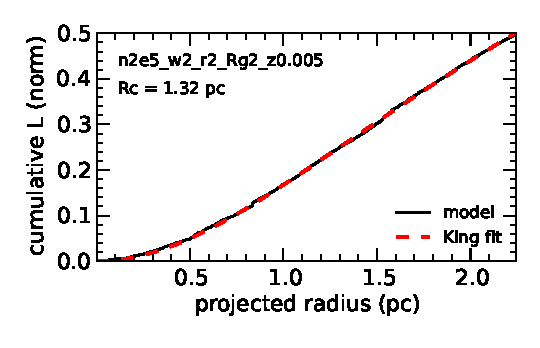
\includegraphics[width=\textwidth]{./plots/n2e5_sbp/kingfit_r3.eps}
                \caption{r3}
                \label{fig:mouse}
        \end{subfigure}
       
       
        \begin{subfigure}[b]{0.3\textwidth}
                \includegraphics[width=\textwidth]{./plots/n2e5_sbp/kingfit_r4.eps}
                \caption{r4}
                \label{fig:gull}
        \end{subfigure}%
        ~ %add desired spacing between images, e. g. ~, \quad, \qquad etc.
          %(or a blank line to force the subfigure onto a new line)
        \begin{subfigure}[b]{0.3\textwidth}
                \includegraphics[width=\textwidth]{./plots/n2e5_sbp/kingfit_r5.eps}
                \caption{r5}
                \label{fig:tiger}
        \end{subfigure}
        ~ %add desired spacing between images, e. g. ~, \quad, \qquad etc.
          %(or a blank line to force the subfigure onto a new line)
        \begin{subfigure}[b]{0.3\textwidth}
                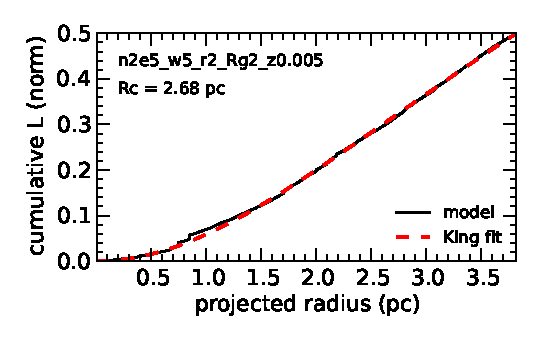
\includegraphics[width=\textwidth]{./plots/n2e5_sbp/kingfit_r6.eps}
                \caption{r6}
                \label{fig:mouse}
        \end{subfigure}

       \begin{subfigure}[b]{0.3\textwidth}
                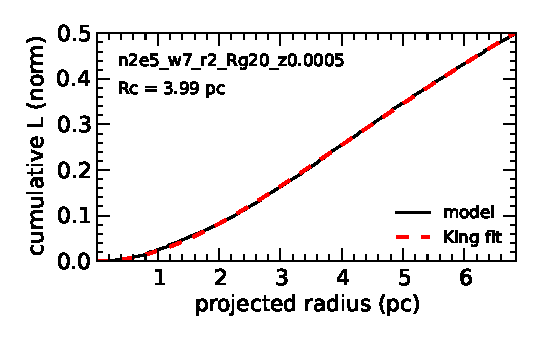
\includegraphics[width=\textwidth]{./plots/n2e5_sbp/kingfit_r7.eps}
                \caption{r7}
                \label{fig:gull}
        \end{subfigure}%
        ~ %add desired spacing between images, e. g. ~, \quad, \qquad etc.
          %(or a blank line to force the subfigure onto a new line)
        \begin{subfigure}[b]{0.3\textwidth}
                \includegraphics[width=\textwidth]{./plots/n2e5_sbp/kingfit_r8.eps}
                \caption{r8}
                \label{fig:tiger}
        \end{subfigure}
        ~ %add desired spacing between images, e. g. ~, \quad, \qquad etc.
          %(or a blank line to force the subfigure onto a new line)
        \begin{subfigure}[b]{0.3\textwidth}
                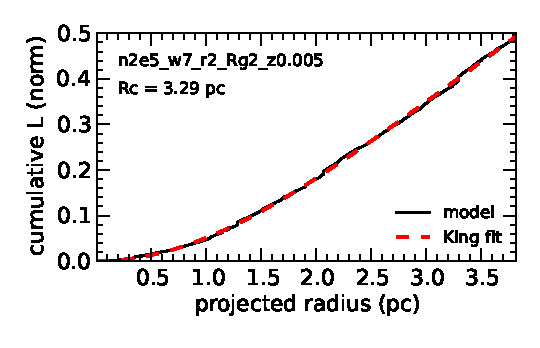
\includegraphics[width=\textwidth]{./plots/n2e5_sbp/kingfit_r9.eps}
                \caption{r9}
                \label{fig:mouse}
        \end{subfigure}

        \caption{``Observational" core radius fits for  $N = 2\times 10^5$ star models.}\label{fig:animals}
\end{figure}




\begin{figure}
        \centering

        \begin{subfigure}[b]{0.3\textwidth}
                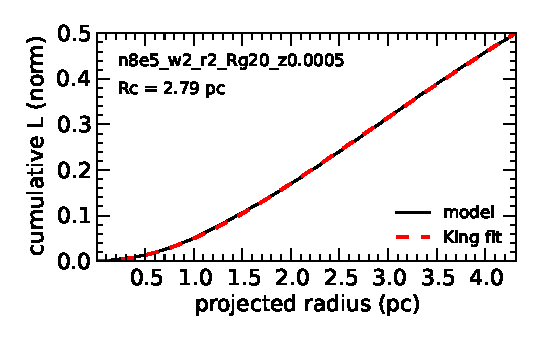
\includegraphics[width=\textwidth]{./plots/n8e5_sbp/kingfit_r10.eps}
                \caption{r10}
                \label{fig:gull}
        \end{subfigure}%
        ~ %add desired spacing between images, e. g. ~, \quad, \qquad etc.
          %(or a blank line to force the subfigure onto a new line)
        \begin{subfigure}[b]{0.3\textwidth}
                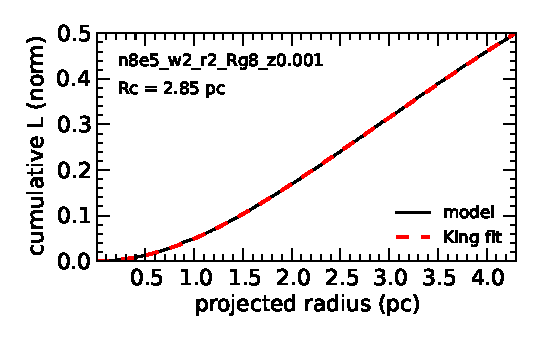
\includegraphics[width=\textwidth]{./plots/n8e5_sbp/kingfit_r11.eps}
                \caption{r11}
                \label{fig:tiger}
        \end{subfigure}
        ~ %add desired spacing between images, e. g. ~, \quad, \qquad etc.
          %(or a blank line to force the subfigure onto a new line)
        \begin{subfigure}[b]{0.3\textwidth}
                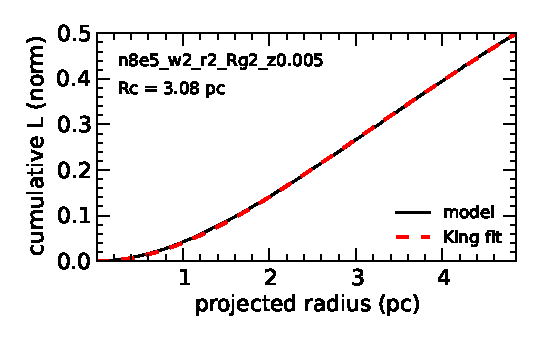
\includegraphics[width=\textwidth]{./plots/n8e5_sbp/kingfit_r12.eps}
                \caption{r12}
                \label{fig:mouse}
        \end{subfigure}
       
       
        \begin{subfigure}[b]{0.3\textwidth}
                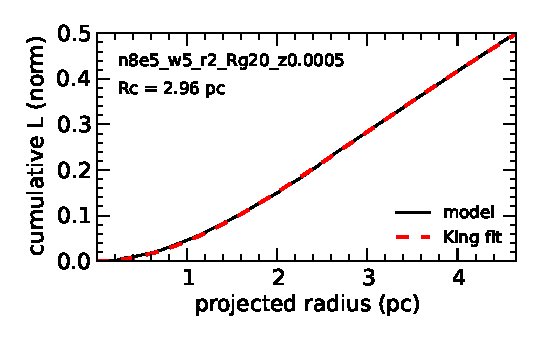
\includegraphics[width=\textwidth]{./plots/n8e5_sbp/kingfit_r13.eps}
                \caption{r13}
                \label{fig:gull}
        \end{subfigure}%
        ~ %add desired spacing between images, e. g. ~, \quad, \qquad etc.
          %(or a blank line to force the subfigure onto a new line)
        \begin{subfigure}[b]{0.3\textwidth}
                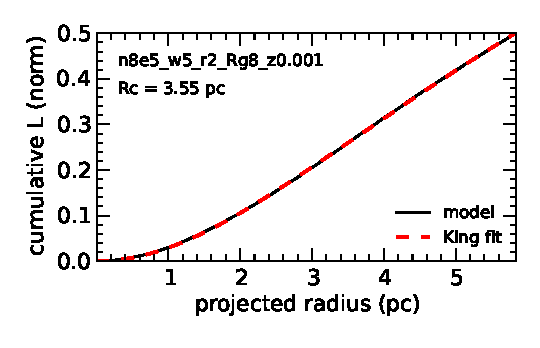
\includegraphics[width=\textwidth]{./plots/n8e5_sbp/kingfit_r14.eps}
                \caption{r14}
                \label{fig:tiger}
        \end{subfigure}
        ~ %add desired spacing between images, e. g. ~, \quad, \qquad etc.
          %(or a blank line to force the subfigure onto a new line)
        \begin{subfigure}[b]{0.3\textwidth}
                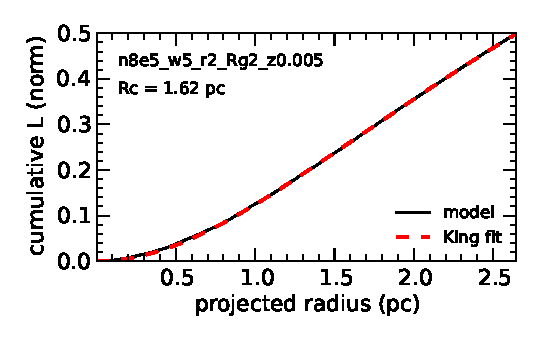
\includegraphics[width=\textwidth]{./plots/n8e5_sbp/kingfit_r15.eps}
                \caption{r15}
                \label{fig:mouse}
        \end{subfigure}

       \begin{subfigure}[b]{0.3\textwidth}
                \includegraphics[width=\textwidth]{./plots/n8e5_sbp/kingfit_r16.eps}
                \caption{r16}
                \label{fig:gull}
        \end{subfigure}%
        ~ %add desired spacing between images, e. g. ~, \quad, \qquad etc.
          %(or a blank line to force the subfigure onto a new line)
        \begin{subfigure}[b]{0.3\textwidth}
                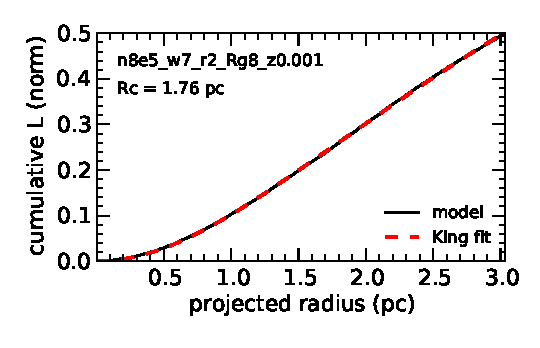
\includegraphics[width=\textwidth]{./plots/n8e5_sbp/kingfit_r17.eps}
                \caption{r17}
                \label{fig:tiger}
        \end{subfigure}
        ~ %add desired spacing between images, e. g. ~, \quad, \qquad etc.
          %(or a blank line to force the subfigure onto a new line)
        \begin{subfigure}[b]{0.3\textwidth}
                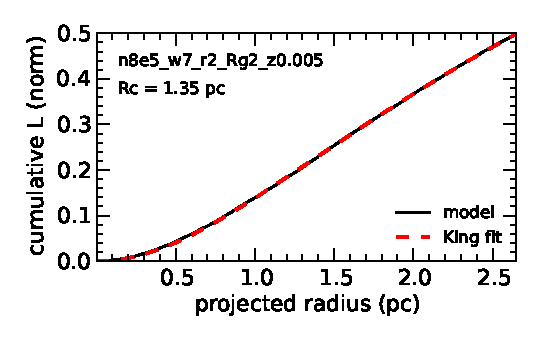
\includegraphics[width=\textwidth]{./plots/n8e5_sbp/kingfit_r18.eps}
                \caption{r18}
                \label{fig:mouse}
        \end{subfigure}

        \caption{``Observational" core radius fits for $N=8 \times 10^5$ star models.}\label{fig:animals}
\end{figure}





\bibliographystyle{hapj} \bibliography{mybibtex}


\end{document}



%\begin{abstract}
%Globular clusters should be born with significant numbers of
%stellar-mass black holes (BHs). It has been thought for two decades
%that very few of these BHs could be retained through the cluster
%lifetime. With masses $\sim 10\, M_\odot$, BHs are $\sim$ 20 times
%more massive than an average cluster star.  They segregate into the
%cluster core, where they may eventually decouple from the remainder of
%the cluster.  The small-$N$ core then evaporates on a short timescale.
%This is the so-called Spitzer instability.  Here we present the
%results of a full dynamical simulation of a globular cluster
%containing many stellar-mass BHs with a realistic mass spectrum. Our
%Monte Carlo simulation code includes detailed treatments of all
%relevant stellar evolution and dynamical processes. Our main finding
%is that old globular clusters could still contain many BHs at
%present. In our simulation, we find no evidence for the Spitzer
%instability. Instead, most of the BHs remain well-mixed with the rest
%of the cluster, with only the innermost few tens of BHs segregating
%significantly. Over the 12 Gyr evolution, fewer than half of the BHs
%are dynamically ejected through strong binary interactions in the
%cluster core. The presence of BHs leads to long-term heating of the
%cluster, ultimately producing a core radius on the high end of the
%distribution for Milky Way globular clusters (and those of other
%galaxies). A crude extrapolation from our model suggests that the
%BH--BH merger rate from globular clusters could be comparable to the
%rate in the field.
%
%%
%\end{abstract}
%
%\keywords{binaries: close --- globular clusters: general --- Gravitational waves ---  Methods: numerical --- Stars: kinematics and dynamics}
%
%
% %%%%%%%%%%%%%%%%%%%%%%%%%%%%%%%%%%%%%%%%%%%%%%%%%%%%%%%
%
%\section{Introduction} \label{Intro}
%
%Typical globular clusters (GCs) should form $\sim 100\, -\, 1000$ BHs
%within $\sim$ 3 Myr and could retain most of them initially, if their natal 
%kicks are sufficiently low (see \citealt{Wong2012} and references therein).  
%With masses $\sim 10\, M_\odot$, these BHs become the most massive 
%objects in the cluster after just $\sim 10\,$Myr, so their dynamics will be very
%different than that of typical stars.  The presence of BHs can affect
%the overall structure and evolution of the parent cluster
%\citep{Mackey2008}.  BHs accreting from a stellar companion can be
%visible as bright X-ray binaries (XRBs), which are in principle
%detectable both in our own and other nearby galaxies
%\citep{Kalogera2004}. Merging BH--BH binaries are key sources of
%gravitational waves (GW) which should be detectable by upcoming
%interferometers such as Advanced LIGO \citep{HarryLIGO2010}.
%
%It is well known that the formation rate per unit mass of XRBs is
%higher in clusters by orders of magnitude compared to the field (e.g.,
%\citealt{Pooley2003}). This indicates that dynamics must play an
%essential role in producing cluster XRBs. Prior to 2007, however,
%there had not been a single detection of a \emph{black hole} XRB
%inside a GC, although many had been identified in galactic
%fields. This appeared to agree with many theoretical studies
%suggesting that essentially all BHs within a star cluster should be
%ejected through dynamical interactions on a timescale $\sim 10^9\,$yr
%\citep{Kulkarni1993, Sigurdsson1993, PortegiesZwart2000, OLeary2006,
%  Banerjee2010}.  Key to all these previous studies is the expectation
%that BHs will segregate rapidly through dynamical friction, on a
%timescale $\sim 100\,$Myr, and will succumb to the so-called Spitzer
%instability \citep{Spitzer1969, Kulkarni1993}, i.e., dynamically
%decouple from the cluster by forming a central subcluster consisting
%primarily of BHs. The relaxation time for this small-$N$ sub-cluster
%of BHs is very short, leading to prompt core collapse and evaporation.
%Through dynamical interactions, some BHs will be ejected in the form
%of tight BH--BH binaries that merge via GW emission within a Hubble time.
%
%This scenario was first proposed based on simple analytic estimates by
%\cite{Kulkarni1993} and \cite{Sigurdsson1993}.  The first direct
%$N$-body simulations of this effect used up to $N\sim 10^4$ particles
%(e.g., \citealt{PortegiesZwart2000,Merritt2004}).  Larger direct
%$N$-body simulations by \cite{Banerjee2010} used $N\sim 10^5$, but
%with a single black hole mass ($10\,M_\odot$) and no primordial
%binaries.  Using simple dynamical models, \citet{OLeary2006} and
%\citet{Sadowski2008} studied the evolution of populations of BHs that
%were either completely decoupled from or in equilibrium with the
%cluster, respectively (see discussion in \citealt{Downing2010a}).
%
%Monte Carlo (MC) methods have made it possible to model realistic GCs
%\emph{self-consistently} with $N\sim 10^5 - 10^6$ and significant
%primordial binary fractions (e.g., \citealt{Giersz2008},
%\citealt{Chatterjee2010}).  The most realistic GC models with BHs to
%date are from \cite{Downing2010a, Downing2011b}, who used a
%H{\'e}non-type MC code to simulate clusters with $N = 5\times 10^5$
%stars, a distribution of BH masses, and primordial binaries.  These
%works used analytic cross sections to determine the results of
%dynamical interactions, rather than direct integration.
%
%Previous studies suggest that most BHs are ejected on a timescale
%$\sim 10^9\,$yr.  Hence, old GCs should have very few, if any, BHs
%left. However, in 2007 the first candidate BH XRB \emph{inside} a GC
%was detected in NGC 4472 \citep{MaccaroneNature2007}.  Since then,
%several additional BH candidates have been found in clusters in other
%galaxies \citep{Brassington2010, Shih2010, Barnard2011,
%  Maccarone2011}.  \citet{Strader2012} discovered two stellar-mass BHs
%in a \emph{Milky Way} (MW) GC (M22).  Assuming these BHs are accreting
%from white dwarf (WD) companions, and using calculated formation and
%survival rates from \cite{Ivanova2010}, \citet{Strader2012} estimate
%that M22 has $\sim 5-100$ BHs.
%
%Furthermore, there have been a few recent theoretical suggestions that
%significant numbers of BHs could still remain in some old clusters
%\citep{Mackey2008,Moody2009}.  \citet{Mackey2008} used $N$-body
%simulations with BHs to explain the radius-age trend in the clusters
%in the Magellanic Clouds; with different initial retention fractions
%for BHs, they were able to reproduce the trend of increasing spread in
%core radius with age in these systems. In some models, they retained 
%up to $\simeq 100$ BHs over a Hubble time. 
%% Ask will about "tens"
%%Mention how many BHs they retain, since I mention this paper as evidence FOR BHs in old clusters.
% 
%Here we re-examine the BH retention question based on a realistic,
%large-$N$, fully self-consistent MC model.  We find that that at least
%some old MW clusters may indeed retain a large fraction of their
%primordial BHs. This dramatically different picture for the fate of
%BHs in GCs may have implications for both BH XRBs and the production of
%merging BH--BH binaries.
%
% %%%%%%%%%%%%%%%%%%%%%%%%%%%%%%%%%%%%%%%%%%%%%%%%%%%%%%%
% 
%\section{Method}
%
%We use a H{\'e}non-type MC method to self-consistently model the
%evolution of star clusters due to the effects of two-body relaxation,
%strong binary scattering encounters, stellar collisions, single and
%binary stellar evolution, and mass loss from the Galactic tidal field.
%A detailed description of our code, as well as examples of its
%capabilities and comparisons with other methods, can be found in
%\citet{Joshi2000, Joshi2001, Fregeau2003, Fregeau2007,
%  Chatterjee2010}. The code has been well tested against direct
%$N$-body models whenever possible.  Since the dynamical evolution of
%BHs in clusters is strongly dependent on interactions involving BH
%binaries, we perform direct calculations of all strong 3-body
%(binary-single) and 4-body (binary-binary) interactions using the
%small-$N$ integrator {\tt Fewbody} \citep{Fregeau2004}. These interactions
%are responsible for the hardening of BH--BH binaries and ejections of
%BHs from the cluster. Single star and binary evolution are modeled
%using the routines of SSE and BSE
%\citep{Hurley2000,Hurley2002}. Orbital energy loss from GW emission is
%handled within BSE for binaries retained in the cluster.  For ejected
%systems, which are no longer evolved with our code, we use a
%simplified timescale for GW inspiral in the weak field limit
%\citep{Peters1964}.  Neutron stars and BHs receive natal kicks
%with velocities drawn from a Maxwellian distribution with $\sigma$=265
%km s$^{-1}$. For BHs, the kick velocity is lowered according to the
%amount of material that falls back onto the final BH after the
%supernova explosion, according to \cite{Belczynski2002}.
%
%We have recently added to our code a prescription for three-body
%binary formation, which is important for the evolution of BHs
%\citep{Kulkarni1993, Sigurdsson1993, PortegiesZwart2000,OLeary2006,
%  Banerjee2010}.  We follow a similar procedure to
%\citet{Ivanova2005}, \citet{Ivanova2010}, and \citet{OLeary2006} to
%obtain an expression for the binary formation rate as a function of
%hardness ratio
%\begin{equation}
%\eta = \frac{G \, m_1 \, m_2}{r_p \, <m> \, \sigma^2}.
%\label{eq:eta}
%\end{equation}
%We keep both the geometric and gravitational focusing contributions to
%the cross-section (in contrast to \citealt{Ivanova2010}, where the
%geometric part of the cross section for the third star to interact
%with stars 1 and 2 is dropped).  For local number density, $n$, and
%average relative velocity at infinity, $v_{\infty}$, the rate at which
%two stars ($m_1$ and $m_2$) form a binary with hardness $\eta \, \geq
%\, \eta_{\rm min}$ through an interaction with a third star ($m_3$) is
%given by
%\begin{multline}
%\Gamma(\eta \geq \eta_{min}) = \sqrt{2} \pi^2 n^2
%      {v_{\infty}^{-9}} \\ \times (m_1 + m_2)^5 \eta_{\rm min}^{-5.5} (1 + 2
%      \eta_{\rm min}) \\ \times \left[ 1+2 \eta_{\rm min} \left( \frac{ m_1 + m_2 +
%            m_3}{m_1 + m_2 } \right) \right].
%\label{eq:Gamma}
%\end{multline}
%As we expect only dynamically hard binaries to survive
%\citep{Heggie1975}, we only consider the formation of hard binaries
%with $\eta \geq 5 = \eta_{\rm min}$.  We allow three-body binary
%formation only for BHs.  When forming a three-body binary, we choose a
%value for $\eta$ from a distribution according to the differential
%rate, d$\Gamma$/d$\eta$, with lower limit $\eta_{\rm min}$. The rest
%of the properties of the system are calculated from conservation of
%momentum and energy.
%
%We have checked that our MC prescription produces binaries at
%a rate that is in agreement with the analytic rate from
%Eq.\ (\ref{eq:Gamma}). We have also done a set of tests using a direct
%N-body code \citep{Farr2007} to check that our prescription produces
%hard binaries at the correct rate. Using one of our cluster snapshots,
%we integrated our system of BHs for a short period of time with direct
%$N$-body, and compared our binary formation probability prediction to
%the actual binary formation probability in the direct integration. We
%find good agreement with the direct $N$-body trials, which gives us
%confidence that we are actually producing hard binaries at the correct
%rate.
%
% %%%%%%%%%%%%%%%%%%%%%%%%%%%%%%%%%%%%%%%%%%%%%%%%%%%%%%%
% 
%\section{The Evolution of a Cluster with Stellar-Mass Black Holes}
%
%We present the results of a cluster model starting with $N = 3\times
%10^5$ stars following a King profile with $W_0 = 5$, half-mass radius
%$r_h = 2.44$ pc, metallicity of $Z = 0.001$, and initial binary
%fraction $f_b$ = 0.1.  We choose our stellar masses from the
%\cite{Kroupa2001} initial mass function ranging from 0.1 --
%100$\, M_\odot$. The cluster has initial total mass $M_{\rm tot} =
%2.03 \times 10^5\, M_\odot$ and half-mass relaxation time $T_{\rm rh}
%\approx 6.5 \times 10^8$ yr. The central escape speed 
%is\footnote{Our cluster is well below the velocity dispersion 
%limit of $\sim 40$ km s$^{-1}$ found in \cite{Miller2012}, above which 
%growth of a massive BH through successive mergers might occur.} 
%31 km s$^{-1}$. 
%Only about 12\% of the BHs formed in the cluster received natal kick 
%speeds above this value. We choose our remnant masses according to
%\cite{Belczynski2002}, which produces BH masses in the range 
%$\sim 5-30\, M_\odot$ for $Z=0.001$.
%%which produces a range of BH masses with
%%maximum mass $\sim 30\, M_\odot$ for our metallicity.  
%We form about 700 BHs in total, of which about 600 are retained
%initially (the remainder are ejected by natal kicks). The BH mass
%distribution at an early time is shown in Figure \ref{fig:bh_hist}.
%
%% NOTES FOR MYSELF: I use \approx for the number of BHs bc, for the
%%total #, I find the timstep that has the largest # bhs ret in cluster
%%over all time (timestep 152= 11 Myr)) = 600, then I find from
%%bh_escapers file, how many have been ejected up to that time =
%%94. But, there could have been some stars that would have formed BHs
%%and merged, finally forming 1 instead of 2 bhs (so basically the BH
%%pop. could have been affected by some dynamics, so it is not purely
%%the pop. that would form in isolation from IMF). But, since this time
%%is at step 152=11 Myr, presumably all BHs formed (assumed, since at
%%this time, the # ret BHs is at its largest), yet very little dynamics
%%should have occurred for BHs
%
%%% Add central density to these results!!!!
%
%%The best examples are NGC 6101, with $M_{\rm tot}$ = 1.32$\times10^5$
%%$M_\odot$ and $r_{\rm c}$ = 5.01 pc; IC 4499, with $M_{\rm tot}$ =
%%1.66$\times 10^5$ $M_\odot$; and $r_{\rm c}$ = 5.37 pc; and Rup 106,
%%with $M_{\rm tot}$ = 8.42$\times 10^4$ $M_\odot$ and $r_{\rm c}$ =
%%5.75 pc (Add references here). Thus, our cluster is not a
%%particularly special or extreme case, and so we believe that the
%%following results may be fairly typical for old GCs, in the Milky Way
%%and beyond.
%
%Within a few Myr, the BHs begin to segregate, leading to a central
%collapse by about 400 Myr. Formation of three-body binaries and their
%subsequent interactions lead to repeated core oscillations (see Figure
%\ref{fig:lagrad}).  After about 300 Myr, strong binary interactions
%involving the mass-segregated BH population start to become
%dynamically important, and the rate of ejection of BHs (both single
%and binary) increases abruptly. Ejections continue through the end of
%the simulation, but the rate slows down over time. The evolution of
%the numbers of single and binary BHs retained in and ejected from the
%cluster is shown in Figure \ref{fig:bhs_time_evol}.  For the entire
%simulation, most of the BHs are \emph{single}; in fact, beyond about
%300 Myr, there are typically no more than about 10 BH-binaries in the
%cluster.
%
%Statistics of the BHs at different times are shown in Table
%\ref{table:BHproperties}.  By 12 Gyr, the cluster has ejected 202
%single BHs, 33 BH--BH binaries, and 6 BH binaries with non-BH
%companions. Throughout the simulation, 13 BH--BH binaries merge due to
%GW emission; 6 of these mergers occur within the cluster, while the
%rest occur post-ejection.  Most of the BH ejections and BH--BH mergers
%occur within about the first 6 Gyr of evolution. At 12 Gyr, our
%model still has nearly 400 BHs, more than half of the
%initially-retained population.
%
%In Figure \ref{fig:cum_fractions} we show the fractions of
%single BHs and all single stars in radial bins at several times.  
%The BH fraction in the central bin, which always contains 20 BHs,
%grows to unity within about 600 Myr (left three panels), 
%%
%meaning that the innermost 20 objects are \emph{all} BHs. 
%%beyond the central bin, the BH fraction tends to decrease radially.
%%This indicates that the BHs are segregating, as expected.
%Just outside the central bin,
%the BH fraction is typically less than 0.4, and it decreases to 
%negligible fractions beyond about 1 pc.
% %
% This indicates that, while the BHs do
%indeed segregate to some extent, most of the BHs \emph{do not}
%dynamically decouple from the cluster (i.e.\ they do not become
%Spitzer unstable). All but the innermost 20 or so most massive BHs
%remain well mixed with the cluster at all times.
%
%The most massive BHs tend to be preferentially ejected from the
%cluster (see Figure \ref{fig:bh_hist} and Table
%\ref{table:BHproperties}). Nearly 75\% of the ejected BHs have masses
%$\gtrsim 20\, M_\odot$, despite the fact that these more massive BHs
%are much less common than lower mass BHs. Since the most massive BHs
%sink the deepest, they tend to have the highest rates of strong
%interactions, which provide the energy needed to eject them from the
%cluster.
%
%We end at 12 Gyr, a typical age for MW GCs, with the cluster having $N
%= 2.47\times 10^5$ stars, $M_{\rm tot} = 1.05\times 10^5\,M_\odot$,
%$r_h$ = 12.7 pc, and binary fraction $f_b$ = 0.098.  The final mass of
%our cluster is just slightly larger than the median value for MW GCs
%($M_{med}\approx 8 \times 10^4$; \citealt{HeggieHut2003}).  For our
%model we find an observational core radius, $r_c \simeq 5-7$ pc, which
%falls within the high end of the core radius distribution of the MW GC
%system, and is also consistent with the range of core radii associated
%with old ($\sim 10$ Gyr) GCs in the Magellanic Clouds (see Figures 1
%and 2 in \citealt{Mackey2008}).
%
% %%%%%%%%%%%%%%%%%%%%%%%%%%%%%%%%%%%%%%%%%%%%%%%%%%%%%%%
% 
%%\section{Discussion}
%\section{Discussion and Conclusions}
%
%The evolution and survivability of BHs in clusters, as well the effect
%that BHs have on their host cluster, will depend strongly on the
%degree to which the BHs are able to decouple from the cluster.  Our MC
%method allows us to include realistic initial conditions as well as
%all the relevant physics for studying these types of systems in
%detail.  
%
%In the most optimistic model of \citet{Mackey2008} (\texttt{run 4}),
%about 50\% of their BHs ($\approx 100$) are retained over $\sim 10$
%Gyr. This is slightly less than our final retention fraction (about 65
%\%), but with $N$ of three times that of \citet{Mackey2008}, this
%amounts to more than a factor of three difference in the actual
%\emph{number} of BHs that we retain.  In contrast with
%\citet{Mackey2008} who found no BH--BH mergers within a Hubble time,
%we produce 13 mergers.  In clusters with low central escape
%velocities, recoil kicks from strong dynamical encounters may tend to
%eject BH-BH binaries before they are tight enough to merge within a
%Hubble time. Although some of the Mackey et al. (2008) models do
%indeed have significantly lower escape velocities than the model we
%present, their \texttt{run 4} actually has a comparable escape velocity, so
%this cannot reconcile the difference in merger rate.  
%%Instead, the discrepancy may be explained by the larger number of BHs, 
%%as well as the inclusion of primordial binaries, in our simulation.
%Instead, the discrepancy may be explained by the larger number of BHs,
% as well as the inclusion of primordial binaries, resulting in a 
% higher interaction rate in our simulation, which is consistent with the larger 
% number of ejected BHs
%%Additionally, our cluster likely has a higher interaction rate.
%%A higher interaction rate 
%% Next sentence is obvious, I guess...
%%which may lead to the formation of tighter BH--BH
%%binaries, and hence, a larger number of mergers 
%(but see discussion in
%\cite{Downing2010a} about the competing effects of \emph{hardening}
%and \emph{destruction} of BH--BH binaries, that go along with high BH
%interaction rates).  We also compare to \cite{Downing2010a}, who track
%BH--BH mergers in a set of MC simulations. Their model
%\texttt{10low75} is most similar to ours, with the same binary
%fraction and metallicity, and $N = 5 \times 10^5$, $r_{\rm h}$ = 2 pc
%and $T_{\rm rh}$ = 5.25 $\times 10^8$ yr. They produced 6 $\pm$ 3
%mergers (averaged over 10 simulations) within $T_H$, about half as
%many as we produce in our simulation.  Agreement to within a factor of
%two is reasonable, considering their use of cross sections for
%predicting the outcomes of strong binary interactions (rather than
%direct integration), which may overestimate the disruption rate for
%tight BH--BH binaries \citep{Downing2010a}.
%
%A crude extrapolation from our model can be used to estimate the rate
%of BH--BH mergers in a Milky Way equivalent galaxy (MWEG). In our
%model, the total merger rate is $\sim 1$ per Gyr.  Our Galaxy may have
%had $\sim 300$ GCs (about half of which have since dissolved). We
%therefore estimate a merger rate of $\sim0.3$ per MWEG per Myr from
%star clusters. This is exceeds the estimated merger rate from
%primordial binaries in the galactic field \citep{Abadie2010}. Thus,
%our model indicates that it is important to include GCs in
%calculations of the BH--BH merger rate of the Universe.
%
%Our results indicate that at least \emph{some} old GCs could have
%\emph{hundreds} of stellar-mass BHs at present. Since nearly all of
%our BHs are single, our prediction is consistent with the small number
%of BH XRBs detected in clusters to date. This result is timely,
%considering the recent discovery of \emph{two} BH XRBs in a Milky Way
%GC by \cite{Strader2012}, who suggest that there may actually be $\sim
%5-100$ BHs in M22 at present. Our main conclusion is different from that 
%of many other studies in the literature. This difference is not easily reconciled,
% but will be the subject of future investigations.
%
%As has been suggested by \cite{Mackey2008}, the presence of BHs can
%indeed cause heating that can lead to significant core expansion,
%as we confirm with our model.
%%. Our model has a final core size that is on the high end of the
%%distribution for medium-mass MW GCs.  
%The smaller cores observed in 
%MW globulars may indicate larger BH kicks than assumed in this work; 
%intriguingly, \citet{Repetto2012} suggested such a change to the kick distribution 
%on the basis of a population synthesis study of Galactic BHs.  
%
%
%%We plan to perform many more simulations with a wide range of 
%%initial conditions to explore whether it is possible to produce 
%%the compact cores more typical for MW GCs, while still retaining 
%%significant numbers of BHs. We may ultimately be able to use
%%the properties of GCs to constrain BH formation processes, including
%% natal kick and mass distributions.
%% 
%% The dynamics of the retained population of BHs causes significant core expansion in our model. We plan to perform many more simulations across a wide range of cluster parameters to determine how [common] (other word here??) this result is. If we find similar results for clusters with different initial properties, then we will have to address the question of how we can produce the more typical GC core radii of \simeq 1 pc. In this case, we may be able use GC properties to constrain BH formation processes, including natal kick and mass distributions. There has been a recent suggestion that BHs may receive similar kick velocities to neutron stars (Repetto et al. 2012). The mass distribution of BHs is still highly uncertain (references).
%
% %%%%%%%%%%%%%%%%%%%%%%%%%%%%%%%%%%%%%%%%%%%%%%%%%%%%%%%
%
%\begin{figure}
%	\plotone{bh_mass_hist_lowZ.eps}
%	\caption{Mass functions for BHs present \emph{in the cluster}
%          at 0.93 Gyr (solid black line) and at 12 Gyr (dotted grey
%          line). The population at 0.93 Gyr is representative of the
%          original population of \textit{initially retained} BHs, as
%          some (about 100) are ejected from the cluster at formation
%          from natal kicks. Between 0.93--12 Gyr, the most massive ($m_{bh} \geq 20\,
%          M_\odot$) are ejected preferentially over the lower mass BHs
%          because they have higher interaction rates.}
%% The following is in the text instead.
%	%The reason for this is that since the most massive BHs sink
%	%the deepest, they tend to have the highest rates of strong
%	%interactions, which provide the energy needed to eject them
%	%from the cluster.}  Although lower-mass BHs require a lower
%	%momentum kick to allow them to escape, they suffer from lack
%	%of momentum-boosting dynamical encounters because they remain
%	%so well mixed throughout the cluster.}
%	\label{fig:bh_hist}
%
%\end{figure}
%
%\begin{figure}
%\plotone{lagrad_multi_tryagain.eps}
%
%   \caption{Evolution of the Lagrange radii of the BHs and all
%     \emph{other} objects. Plots show the radii enclosing 1\%, 5\%,
%     10\%, and 50\% of the mass, from bottom to top, for each category
%     of object: BHs (solid curves) and non-BH (dotted curves). The left panel 
%     shows the evolution over the shorter interval corresponding to the grey
%     band in the right panel. The BHs segregate from the rest of the cluster 
%     on a timescale of a few hundred Myr. The vertical grey dashed lines
%      indicate the times when three-body binaries form. 
%      Interactions involving these hard binaries cause most of the oscillations 
%      of the innermost Lagrange radii. However, interactions involving 
%      hard binaries \emph{not} created by three-body formation can also 
%      cause the same
%     effect.}
%      \label{fig:lagrad}
%      \end{figure}
%
%
%\begin{figure}
%
%	\plotone{bhs_time_evolution_paper_lowZ.eps}
% 	\caption{Evolution of BH population retained in (top) and
%          ejected from (bottom) the cluster. Each plot shows the
%          number of single BHs (solid black line), BH--BH binaries
%          (dashed red line), and BH-binaries with a \emph{non-BH}
%          companion (dotted blue line), either retained or ejected.
%          The number of BH--BH binaries within the cluster tends to
%          \emph{decrease} over time until there are just a few.  Both
%          single BHs and BH--BH binaries are ejected efficiently from
%          about 300 Myr until about 6 Gyr, at which point the ejection
%          rate slows down significantly.  This occurs in conjunction
%          with a drop in the overall binary interaction rate, which is
%          caused by the ongoing cluster expansion due to heating by
%          the BHs. BH--other binaries tend to increase in number very
%          slowly over time.  At 12 Gyr, the cluster still has 395 BHs,
%          more than half of the cluster's initial population. The
%          majority of the BHs are \emph{single} at all times.}
%	\label{fig:bhs_time_evol}
%
%\end{figure}
%		
%
%
%
%% ADD TO THIS TABLE - COLUMN 1, initial numbers of BHs, m_ave, etc.
%\begin{deluxetable}{c|cc|cc|cc|cc|cc}
%\tablecolumns{11} \tabletypesize{\scriptsize} \tablewidth{0pc}
%\tablecaption{Properties of BH population at different evolutionary
%  stages: 0.93 Gyr, 3.25 Gyr, 6.5 Gyr, 9.77 Gyr and 12 Gyr. The table
%  shows the number of single BHs ($N_{\rm sBH}$), number of BH-BH
%  binaries ($N_{\rm BH-BH}$), number of BH--other (non-compact)
%  binaries ($N_{\rm BH-other}$), number of BHs with masses above 20$\,
%  M_\odot$ ($N_{\rm BH}(m\geq20\, M_\odot)$), average individual BH
%  mass ($m_{\rm ave,BH}$), that are retained in/ejected from the
%  cluster, at the different times.  We also show the number of BH--BH
%  mergers ($N_{\rm mgr}$) that have occurred up to the time given,
%  either inside the cluster or post ejection.}  \tablehead{
%  \multicolumn{1}{c}{type} & \multicolumn{2}{c}{$T=0.93$ Gyr} &
%  \multicolumn{2}{c}{$T=3.25$ Gyr} & \multicolumn{2}{c}{$T=6.50$ Gyr}
%  & \multicolumn{2}{c}{$T=9.77$ Gyr} & \multicolumn{2}{c}{$T=12$ Gyr}
%  \\ \multicolumn{1}{c}{} & \multicolumn{2}{c}{$=1.4\,T_{rh}$} &
%  \multicolumn{2}{c}{$=5\,T_{rh}$} &
%  \multicolumn{2}{c}{$=10\,T_{rh}$} &
%  \multicolumn{2}{c}{$=15\,T_{rh}$} &
%  \multicolumn{2}{c}{$=18.5\,T_{rh}$} \\ \colhead{} &
%  \colhead{ret} & \colhead{ej} & \colhead{ret} & \colhead{ej} &
%  \colhead{ret} & \colhead{ej} & \colhead{ret} & \colhead{ej} &
%  \colhead{ret} & \colhead{ej} }
%
%\startdata
%%									0.93 Gyr				3.25 Gyr			6.5 Gyr			9.77 Gyr			12 Gyr
%$N_{\rm sBH}$ ...........................  & 534 & 89 & 434 & 166 &
%395 & 197 & 387 & 201 & 385 & 202\\ $N_{\rm BH-BH}$
%......................  & 17 & 4 & 1 & 26 & 0 & 32 & 0 & 33 & 0 &
%33\\ $N_{\rm BH-other}$ ....................  & 3 & 6 & 10 & 6 & 8 & 6
%& 9 & 6 & 10 & 6\\ $m_{\rm ave,BH}\, (M_\odot)$ .............. & 16.7
%& 13.3 & 15.6 & 20.6 & 15.1 & 21.8 & 14.9 & 22.0 & 14.9 &
%22.0\\ $N_{\rm BH}(m\geq20\, M_\odot)$ ........  & 178 & 27 & 101 &
%110 & 69 & 143 & 63 & 148 & 63 & 149\\ $N_{\rm mgr}$
%............................  & 4 & 0 & 5 & 1 & 6 & 6 & 6 & 7 & 6 & 7
%\enddata
%\label{table:BHproperties}
%\end{deluxetable}
%
%
%
%%\renewcommand{\tabcolsep}{0cm}
%%
%\begin{figure}
%%\centering
%\plotone{binned_frac_6panels_final.eps}
%%\plotone{cum_binned_frac_tryagain.eps}
%
%\caption{
%%Fractions of different types of objects within the
%  %radial bins at several times. 
%  The fraction of \emph{single BHs} (solid black line) and \emph{all single stars}
%  (dashed red line) at several times; the remainder of the objects are binaries.  
%  The innermost bin contains 20 BHs, and the number of BHs inside 
%  each subsequent bin doubles (40, 80, etc.).
%  The BH fraction in the central bin (containing 20 BHs) reaches unity by
%  about 600 Myr (left panels), and then fluctuates between 0.4--1 for
%  the rest of the simulation (right panels). Beyond the first bin, the
%  BH fraction decreases, reaching negligible fractions beyond
%  about 1 pc.
%  %
%  The vertical grey dashed line shows the extent of the innermost 140 BHs 
%  ($20+40+80=140$ contained within the first three bins),
%  which is at all times less than half of the retained BH population.}
%\label{fig:cum_fractions} 
%\end{figure}
%
%
%
%\acknowledgements
%
%We thank the anonymous referee for many suggestions that improved this paper.
%This work was supported by NSF Grant PHY-0855592 and NASA ATP Grant
%NNX09AO36G.  MM acknowledges support from an NSF GK-12 Fellowship
%funded through NSF Award DGE-0948017 to Northwestern University.  The
%computations in this paper were performed on Northwestern University's
%HPC cluster Quest.
%


%\begin{thebibliography}{42}
%\expandafter\ifx\csname natexlab\endcsname\relax\def\natexlab#1{#1}\fi
%
%\bibitem[{{Abadie} {et~al.}(2010){Abadie}, {Abbott}, {Abbott}, {Abernathy},
%  {Accadia}, {Acernese}, {Adams}, {Adhikari}, {Ajith}, {Allen}, \&
%  et~al.}]{Abadie2010}
%{Abadie}, J. {et~al.} 2010, Classical and Quantum Gravity, 27, 173001,
%  arXiv:1003.2480
%
%\bibitem[{{Banerjee} {et~al.}(2010){Banerjee}, {Baumgardt}, \&
%  {Kroupa}}]{Banerjee2010}
%{Banerjee}, S., {Baumgardt}, H., \& {Kroupa}, P. 2010, \mnras, 402, 371,
%  arXiv:0910.3954
%
%\bibitem[{{Barnard} {et~al.}(2011){Barnard}, {Garcia}, {Li}, {Primini}, \&
%  {Murray}}]{Barnard2011}
%{Barnard}, R., {Garcia}, M., {Li}, Z., {Primini}, F., \& {Murray}, S.~S. 2011,
%  \apj, 734, 79, arXiv:1104.0860
%
%\bibitem[{{Belczynski} {et~al.}(2002){Belczynski}, {Kalogera}, \&
%  {Bulik}}]{Belczynski2002}
%{Belczynski}, K., {Kalogera}, V., \& {Bulik}, T. 2002, \apj, 572, 407,
%  arXiv:astro-ph/0111452
%
%\bibitem[{{Brassington} {et~al.}(2010){Brassington}, {Fabbiano}, {Blake},
%  {Zezas}, {Angelini}, {Davies}, {Gallagher}, {Kalogera}, {Kim}, {King},
%  {Kundu}, {Trinchieri}, \& {Zepf}}]{Brassington2010}
%{Brassington}, N.~J. {et~al.} 2010, \apj, 725, 1805, arXiv:1003.3236
%
%\bibitem[{{Chatterjee} {et~al.}(2010){Chatterjee}, {Fregeau}, {Umbreit}, \&
%  {Rasio}}]{Chatterjee2010}
%{Chatterjee}, S., {Fregeau}, J.~M., {Umbreit}, S., \& {Rasio}, F.~A. 2010,
%  \apj, 719, 915, arXiv:0912.4682
%
%\bibitem[{{Downing} {et~al.}(2010){Downing}, {Benacquista}, {Giersz}, \&
%  {Spurzem}}]{Downing2010a}
%{Downing}, J.~M.~B., {Benacquista}, M.~J., {Giersz}, M., \& {Spurzem}, R. 2010,
%  \mnras, 407, 1946, arXiv:0910.0546
%
%\bibitem[{{Downing} {et~al.}(2011){Downing}, {Benacquista}, {Giersz}, \&
%  {Spurzem}}]{Downing2011b}
%------. 2011, \mnras, 416, 133, arXiv:1008.5060
%
%\bibitem[{{Farr} \& {Bertschinger}(2007)}]{Farr2007}
%{Farr}, W.~M., \& {Bertschinger}, E. 2007, \apj, 663, 1420,
%  arXiv:astro-ph/0611416
%
%\bibitem[{{Fregeau} {et~al.}(2004){Fregeau}, {Cheung}, {Portegies Zwart}, \&
%  {Rasio}}]{Fregeau2004}
%{Fregeau}, J.~M., {Cheung}, P., {Portegies Zwart}, S.~F., \& {Rasio}, F.~A.
%  2004, \mnras, 352, 1, arXiv:astro-ph/0401004
%
%\bibitem[{{Fregeau} {et~al.}(2003){Fregeau}, {G{\"u}rkan}, {Joshi}, \&
%  {Rasio}}]{Fregeau2003}
%{Fregeau}, J.~M., {G{\"u}rkan}, M.~A., {Joshi}, K.~J., \& {Rasio}, F.~A. 2003,
%  \apj, 593, 772, arXiv:astro-ph/0301521
%
%\bibitem[{{Fregeau} \& {Rasio}(2007)}]{Fregeau2007}
%{Fregeau}, J.~M., \& {Rasio}, F.~A. 2007, \apj, 658, 1047,
%  arXiv:astro-ph/0608261
%
%\bibitem[{{Giersz} {et~al.}(2008){Giersz}, {Heggie}, \& {Hurley}}]{Giersz2008}
%{Giersz}, M., {Heggie}, D.~C., \& {Hurley}, J.~R. 2008, \mnras, 388, 429,
%  arXiv:0801.3968
%
%\bibitem[{{Harry} {et~al.}(2010)}]{HarryLIGO2010}
%{Harry}, G.~M., {et~al.} 2010, Classical and Quantum Gravity, 27, 084006
%
%\bibitem[{{Heggie} \& {Hut}(2003)}]{HeggieHut2003}
%{Heggie}, D., \& {Hut}, P. 2003, {The Gravitational Million-Body Problem: A
%  Multidisciplinary Approach to Star Cluster Dynamics}
%
%\bibitem[{{Heggie}(1975)}]{Heggie1975}
%{Heggie}, D.~C. 1975, \mnras, 173, 729
%
%\bibitem[{{Hurley} {et~al.}(2000){Hurley}, {Pols}, \& {Tout}}]{Hurley2000}
%{Hurley}, J.~R., {Pols}, O.~R., \& {Tout}, C.~A. 2000, \mnras, 315, 543,
%  arXiv:astro-ph/0001295
%
%\bibitem[{{Hurley} {et~al.}(2002){Hurley}, {Tout}, \& {Pols}}]{Hurley2002}
%{Hurley}, J.~R., {Tout}, C.~A., \& {Pols}, O.~R. 2002, \mnras, 329, 897,
%  arXiv:astro-ph/0201220
%
%\bibitem[{{Ivanova} {et~al.}(2005){Ivanova}, {Belczynski}, {Fregeau}, \&
%  {Rasio}}]{Ivanova2005}
%{Ivanova}, N., {Belczynski}, K., {Fregeau}, J.~M., \& {Rasio}, F.~A. 2005,
%  \mnras, 358, 572, arXiv:astro-ph/0501131
%
%\bibitem[{{Ivanova} {et~al.}(2010){Ivanova}, {Chaichenets}, {Fregeau},
%  {Heinke}, {Lombardi}, \& {Woods}}]{Ivanova2010}
%{Ivanova}, N., {Chaichenets}, S., {Fregeau}, J., {Heinke}, C.~O., {Lombardi},
%  Jr., J.~C., \& {Woods}, T.~E. 2010, \apj, 717, 948, arXiv:1001.1767
%
%\bibitem[{{Joshi} {et~al.}(2001){Joshi}, {Nave}, \& {Rasio}}]{Joshi2001}
%{Joshi}, K.~J., {Nave}, C.~P., \& {Rasio}, F.~A. 2001, \apj, 550, 691
%
%\bibitem[{{Joshi} {et~al.}(2000){Joshi}, {Rasio}, \& {Portegies
%  Zwart}}]{Joshi2000}
%{Joshi}, K.~J., {Rasio}, F.~A., \& {Portegies Zwart}, S. 2000, \apj, 540, 969,
%  arXiv:astro-ph/9909115
%
%\bibitem[{{Kalogera} {et~al.}(2004){Kalogera}, {King}, \&
%  {Rasio}}]{Kalogera2004}
%{Kalogera}, V., {King}, A.~R., \& {Rasio}, F.~A. 2004, \apjl, 601, L171,
%  arXiv:astro-ph/0308485
%
%\bibitem[{{Kroupa}(2001)}]{Kroupa2001}
%{Kroupa}, P. 2001, \mnras, 322, 231, arXiv:astro-ph/0009005
%
%\bibitem[{{Kulkarni} {et~al.}(1993){Kulkarni}, {Hut}, \&
%  {McMillan}}]{Kulkarni1993}
%{Kulkarni}, S.~R., {Hut}, P., \& {McMillan}, S. 1993, \nat, 364, 421
%
%\bibitem[{{Maccarone} {et~al.}(2007){Maccarone}, {Kundu}, {Zepf}, \&
%  {Rhode}}]{MaccaroneNature2007}
%{Maccarone}, T.~J., {Kundu}, A., {Zepf}, S.~E., \& {Rhode}, K.~L. 2007, \nat,
%  445, 183, arXiv:astro-ph/0701310
%
%\bibitem[{{Maccarone} {et~al.}(2011){Maccarone}, {Kundu}, {Zepf}, \&
%  {Rhode}}]{Maccarone2011}
%------. 2011, \mnras, 410, 1655, arXiv:1008.2896
%
%\bibitem[{{Mackey} {et~al.}(2008){Mackey}, {Wilkinson}, {Davies}, \&
%  {Gilmore}}]{Mackey2008}
%{Mackey}, A.~D., {Wilkinson}, M.~I., {Davies}, M.~B., \& {Gilmore}, G.~F. 2008,
%  \mnras, 386, 65, arXiv:0802.0513
%
%\bibitem[{{Merritt} {et~al.}(2004){Merritt}, {Piatek}, {Portegies Zwart}, \&
%  {Hemsendorf}}]{Merritt2004}
%{Merritt}, D., {Piatek}, S., {Portegies Zwart}, S., \& {Hemsendorf}, M. 2004,
%  \apjl, 608, L25, arXiv:astro-ph/0403331
%
%\bibitem[{{Miller} \& {Davies}(2012)}]{Miller2012}
%{Miller}, M.~C., \& {Davies}, M.~B. 2012, \apj, 755, 81, arXiv:1206.6167
%
%\bibitem[{{Moody} \& {Sigurdsson}(2009)}]{Moody2009}
%{Moody}, K., \& {Sigurdsson}, S. 2009, \apj, 690, 1370, arXiv:0809.1617
%
%\bibitem[{{O'Leary} {et~al.}(2006){O'Leary}, {Rasio}, {Fregeau}, {Ivanova}, \&
%  {O'Shaughnessy}}]{OLeary2006}
%{O'Leary}, R.~M., {Rasio}, F.~A., {Fregeau}, J.~M., {Ivanova}, N., \&
%  {O'Shaughnessy}, R. 2006, \apj, 637, 937, arXiv:astro-ph/0508224
%
%\bibitem[{Peters(1964)}]{Peters1964}
%Peters, P.~C. 1964, Phys. Rev., 136, B1224
%
%\bibitem[{{Pooley} {et~al.}(2003){Pooley}, {Lewin}, {Anderson}, {Baumgardt},
%  {Filippenko}, {Gaensler}, {Homer}, {Hut}, {Kaspi}, {Makino}, {Margon},
%  {McMillan}, {Portegies Zwart}, {van der Klis}, \& {Verbunt}}]{Pooley2003}
%{Pooley}, D. {et~al.} 2003, \apjl, 591, L131, arXiv:astro-ph/0305003
%
%\bibitem[{{Portegies Zwart} \& {McMillan}(2000)}]{PortegiesZwart2000}
%{Portegies Zwart}, S.~F., \& {McMillan}, S.~L.~W. 2000, \apjl, 528, L17,
%  arXiv:astro-ph/9910061
%
%\bibitem[{{Repetto} {et~al.}(2012){Repetto}, {Davies}, \&
%  {Sigurdsson}}]{Repetto2012}
%{Repetto}, S., {Davies}, M.~B., \& {Sigurdsson}, S. 2012, \mnras, 425, 2799,
%  1203.3077
%
%\bibitem[{{Sadowski} {et~al.}(2008){Sadowski}, {Belczynski}, {Bulik},
%  {Ivanova}, {Rasio}, \& {O'Shaughnessy}}]{Sadowski2008}
%{Sadowski}, A., {Belczynski}, K., {Bulik}, T., {Ivanova}, N., {Rasio}, F.~A.,
%  \& {O'Shaughnessy}, R. 2008, \apj, 676, 1162, arXiv:0710.0878
%
%\bibitem[{{Shih} {et~al.}(2010){Shih}, {Kundu}, {Maccarone}, {Zepf}, \&
%  {Joseph}}]{Shih2010}
%{Shih}, I.~C., {Kundu}, A., {Maccarone}, T.~J., {Zepf}, S.~E., \& {Joseph},
%  T.~D. 2010, \apj, 721, 323, arXiv:1007.4768
%
%\bibitem[{{Sigurdsson} \& {Hernquist}(1993)}]{Sigurdsson1993}
%{Sigurdsson}, S., \& {Hernquist}, L. 1993, \nat, 364, 423
%
%\bibitem[{{Spitzer}(1969)}]{Spitzer1969}
%{Spitzer}, Jr., L. 1969, \apjl, 158, L139
%
%\bibitem[{{Strader} {et~al.}(2012){Strader}, {Chomiuk}, {Maccarone},
%  {Miller-Jones}, \& {Seth}}]{Strader2012}
%{Strader}, J., {Chomiuk}, L., {Maccarone}, T.~J., {Miller-Jones}, J.~C.~A., \&
%  {Seth}, A.~C. 2012, \nat, 490, 71, arXiv:1210.0901
%
%\bibitem[{{Wong} {et~al.}(2012){Wong}, {Valsecchi}, {Fragos},
% \& {Kalogera}}]{Wong2012}
%{Wong}, T.~W., {Valsecchi}, F., {Fragos}, T., \&
%  {Kalogera}, V. 2012, \nat, 747, 111, arXiv:1107.5585
%
%\end{thebibliography}
%
%
%
%\end{document}
